\documentclass{beamer}
\usepackage[utf8]{inputenc}
\usepackage{cite}
\usepackage{graphicx}
\usepackage{float}
\usepackage{fontawesome}
\usepackage{multicol}
\usepackage{listings}
\usepackage{url}

\lstset{
    language=Python,
    basicstyle=\ttfamily\footnotesize,
    breaklines=true,
    frame=single,
    numbers=none,
    keywordstyle=\color{red}\bfseries,
    stringstyle=\color{green!60!black},
    commentstyle=\color{gray},
    showstringspaces=false,
    columns=flexible,
    backgroundcolor=\color{gray!10},
}

% Beamer theme settings
\usetheme{CambridgeUS}
\usecolortheme{default}

\title{Coordination of a Multi-Agent System \\for Emergency Response}
\author{Team 05}
\date{\today}

\begin{document}

\begin{frame}
    \titlepage
\end{frame}

% Introduction
\section{Introduction}
\begin{frame}{Introduction}
    \begin{itemize}
        \item \textbf{Objective}: Design the cooperation and coordination mechanisms that will
        be used to solve the emergency response for fire-related emergencies in Lloret de Mar, Girona.
        \item \textbf{Teams Involved}:
            \begin{itemize}
                \item Emergency Services
                \item Firefighters
                \item Medical Services
                \item Public Communications
                \item \textit{Forensics}
            \end{itemize}
        \item \textbf{Overview}:
            \begin{itemize}
                \item For each crew: process definition and Pydantic outputs. 
                \item Agent interactions: flows and routers.
            \end{itemize}
    \end{itemize}
\end{frame}

\section{Crew Processes}
\subsection{Emergency Services}
\begin{frame}{Emergency Services Process and Outputs}
        \begin{minipage}[b]{0.45\textwidth}
            \centering
            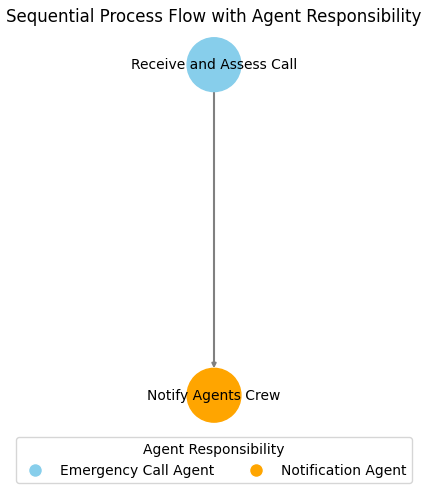
\includegraphics[width=0.75\linewidth]{figures/emergency_services_crew_flow.png}
        \end{minipage}
        \hfill
        \begin{minipage}[b]{0.5\textwidth}
            \begin{itemize}
                \item What type of fire is it?
                \item Where is it? 
                \item Is anyone injured? How badly? 
                \item How severe is the fire? 
                \item Are there hazards? 
                \item Is it an indoor or outdoor fire? 
                \item Is anyone inside or trapped? 
            \end{itemize}
            \vfill
        \end{minipage}
        \centering
            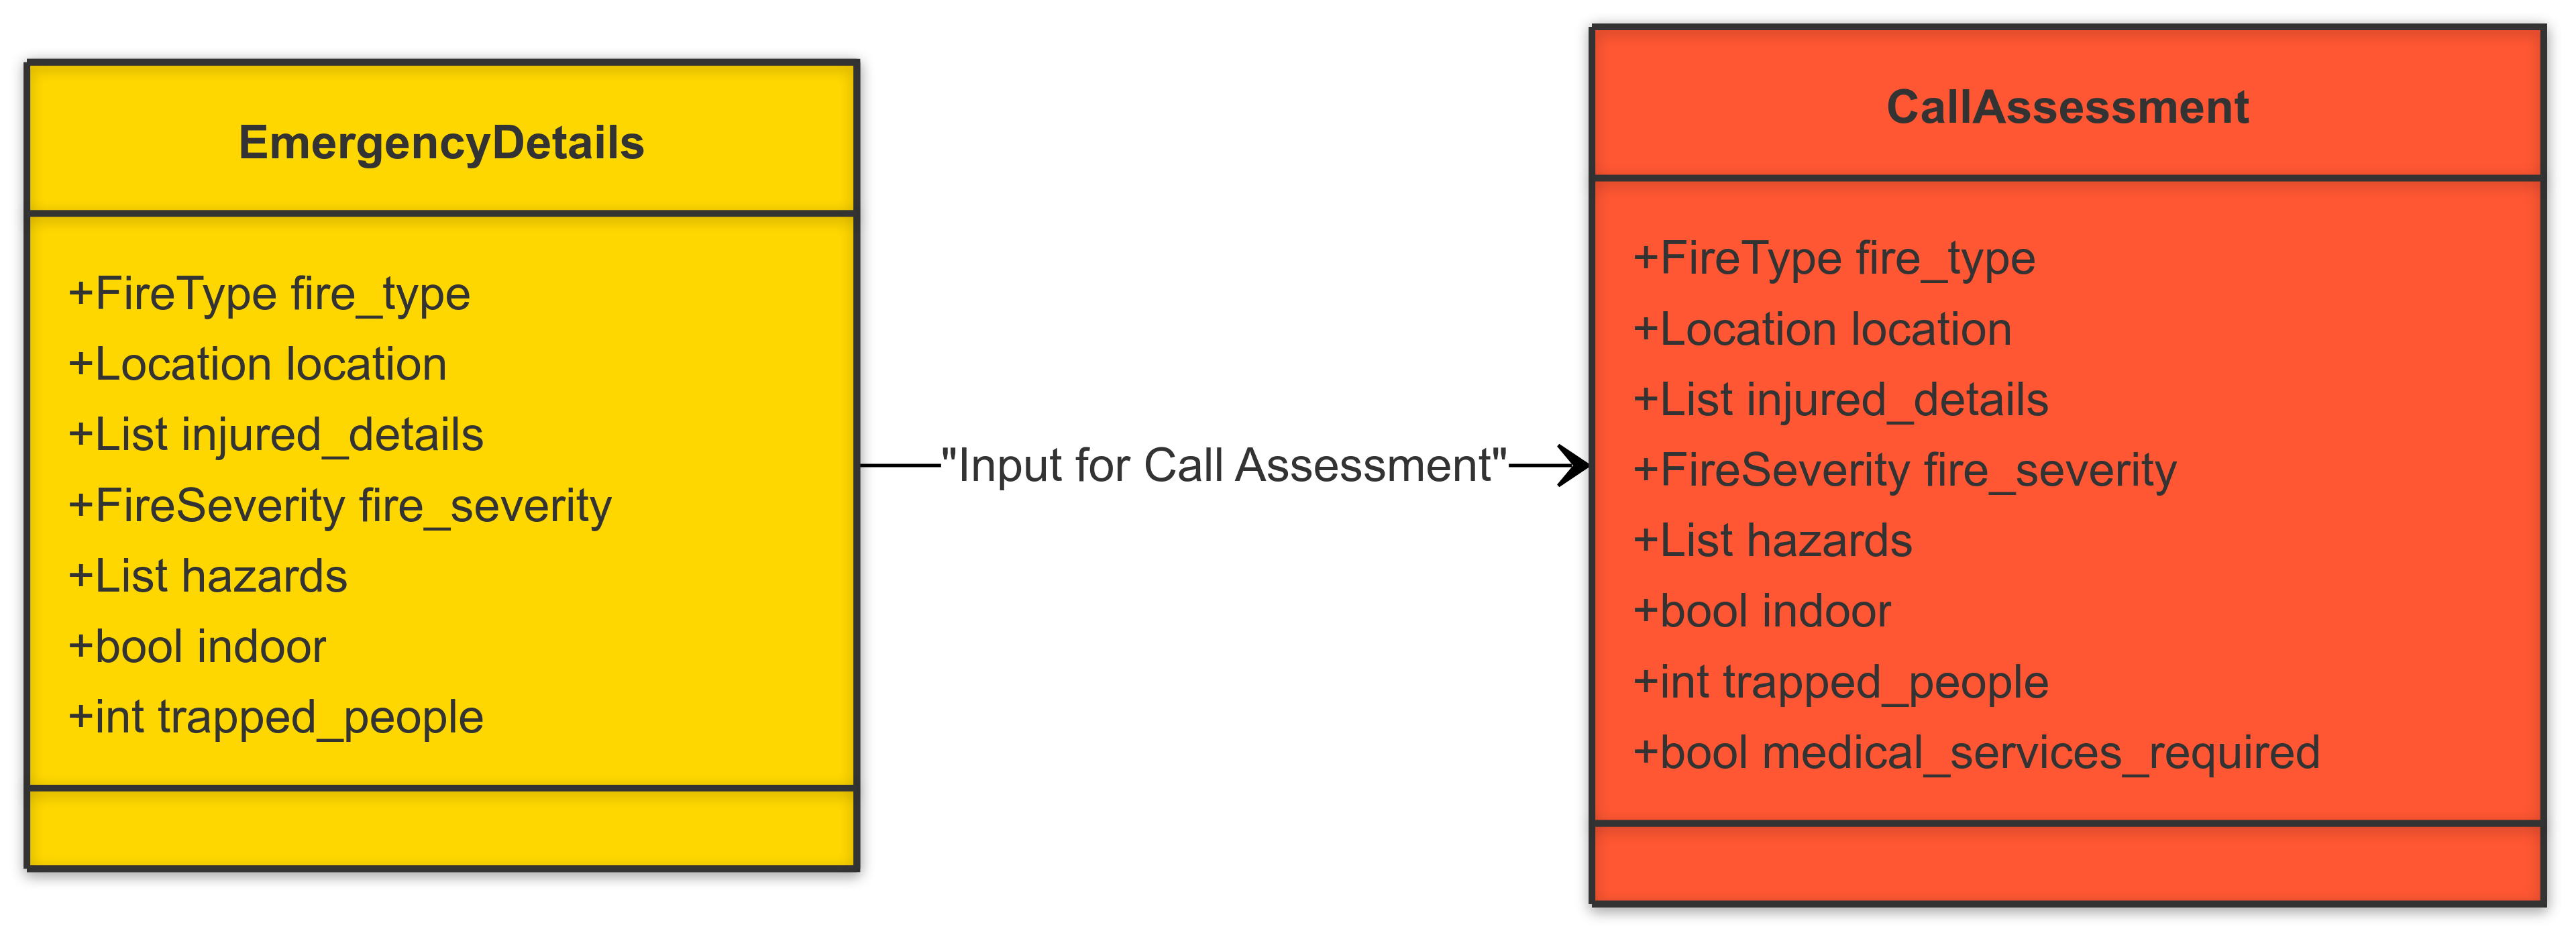
\includegraphics[width=0.7\linewidth]{figures/Emergency-Crew-Diagram.png}
\end{frame}



% Firefighters - Figure 1
\subsection{Firefighters}
\begin{frame}{Firefighters Process}
    \centering
    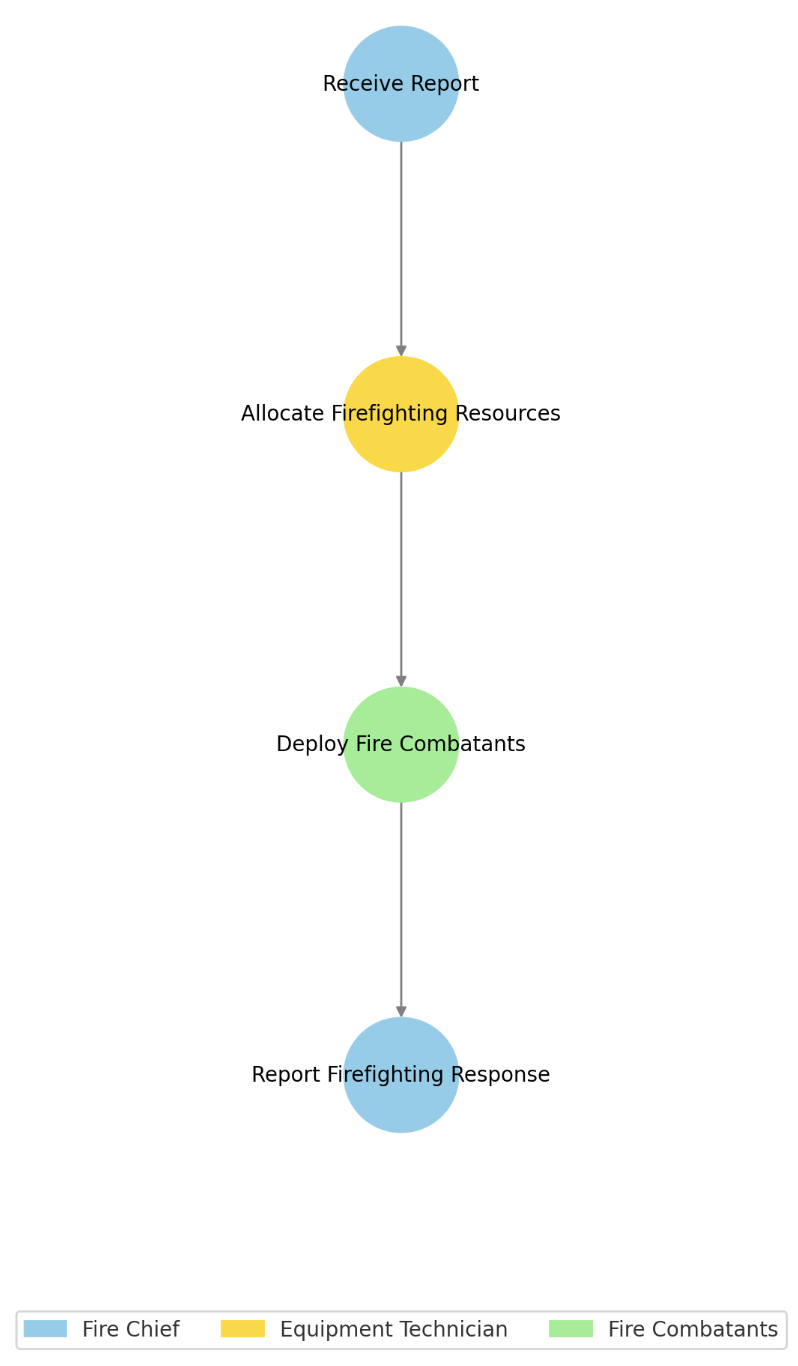
\includegraphics[height=\textheight]{figures/Firefighter_Crew_Flow.png}
\end{frame}

% Firefighters - Figure 2
\begin{frame}{Firefighters Outputs}
    \centering
    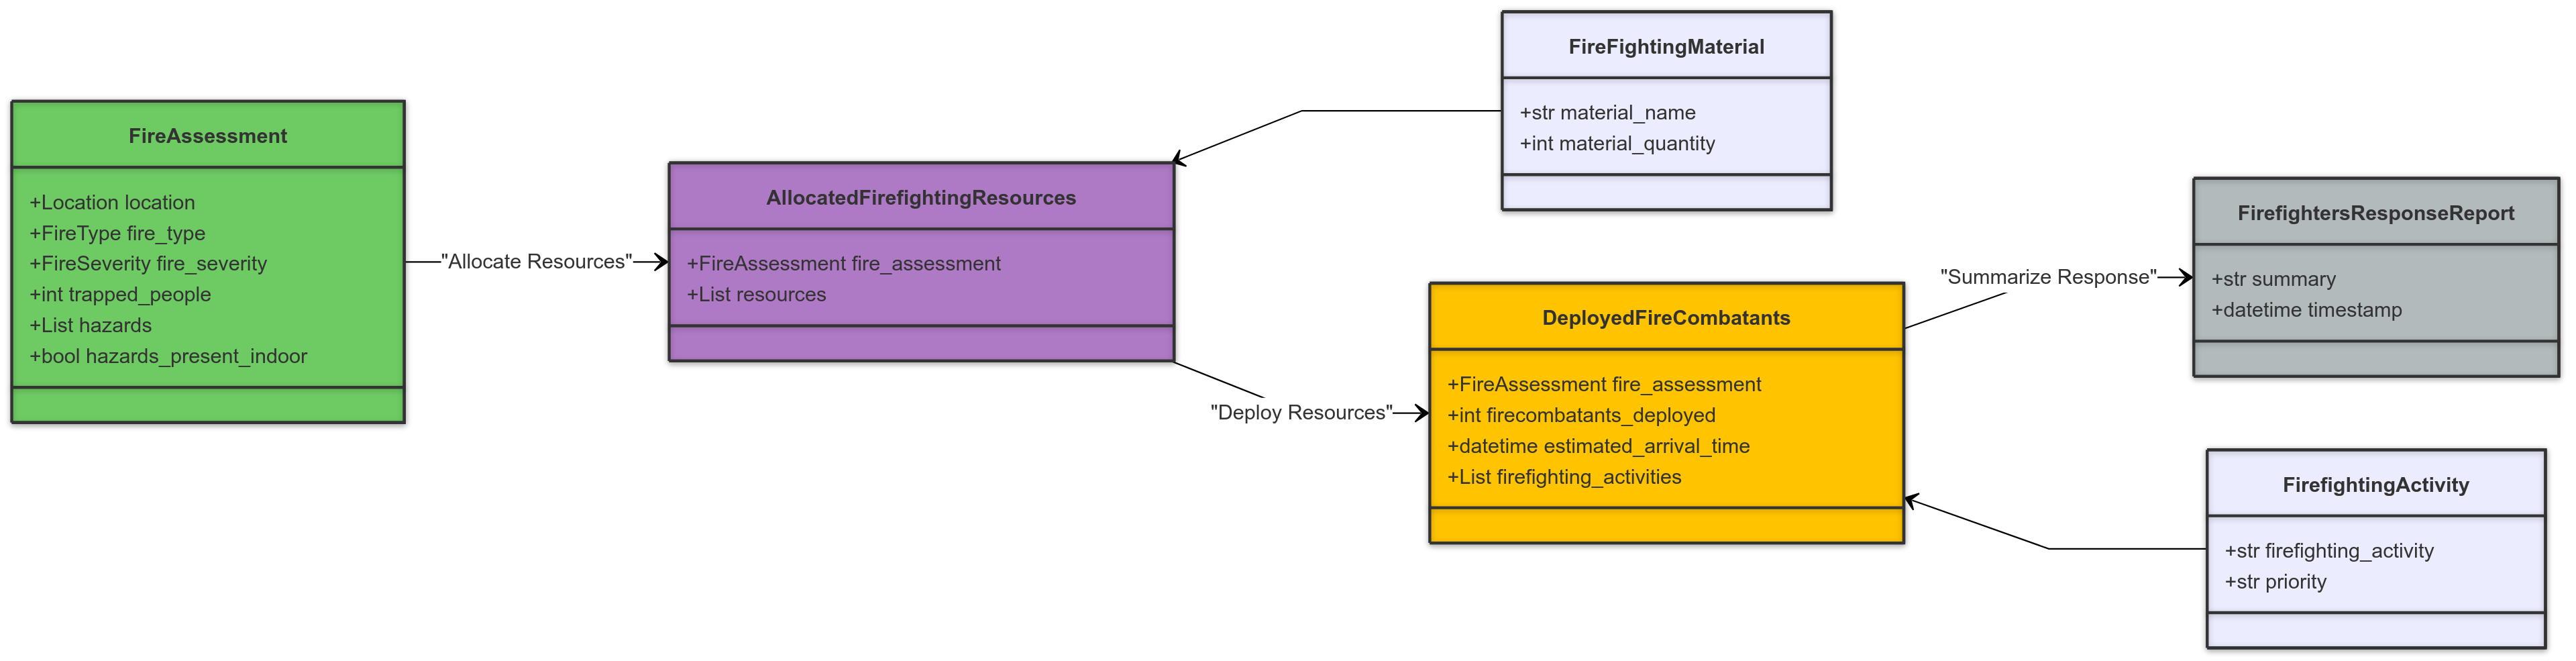
\includegraphics[width=\textwidth]{figures/Firefighters_ClassDiagram.png}
\end{frame}
% Medical Services - Figure 1
\begin{frame}{Medical Services Process}
    \centering
    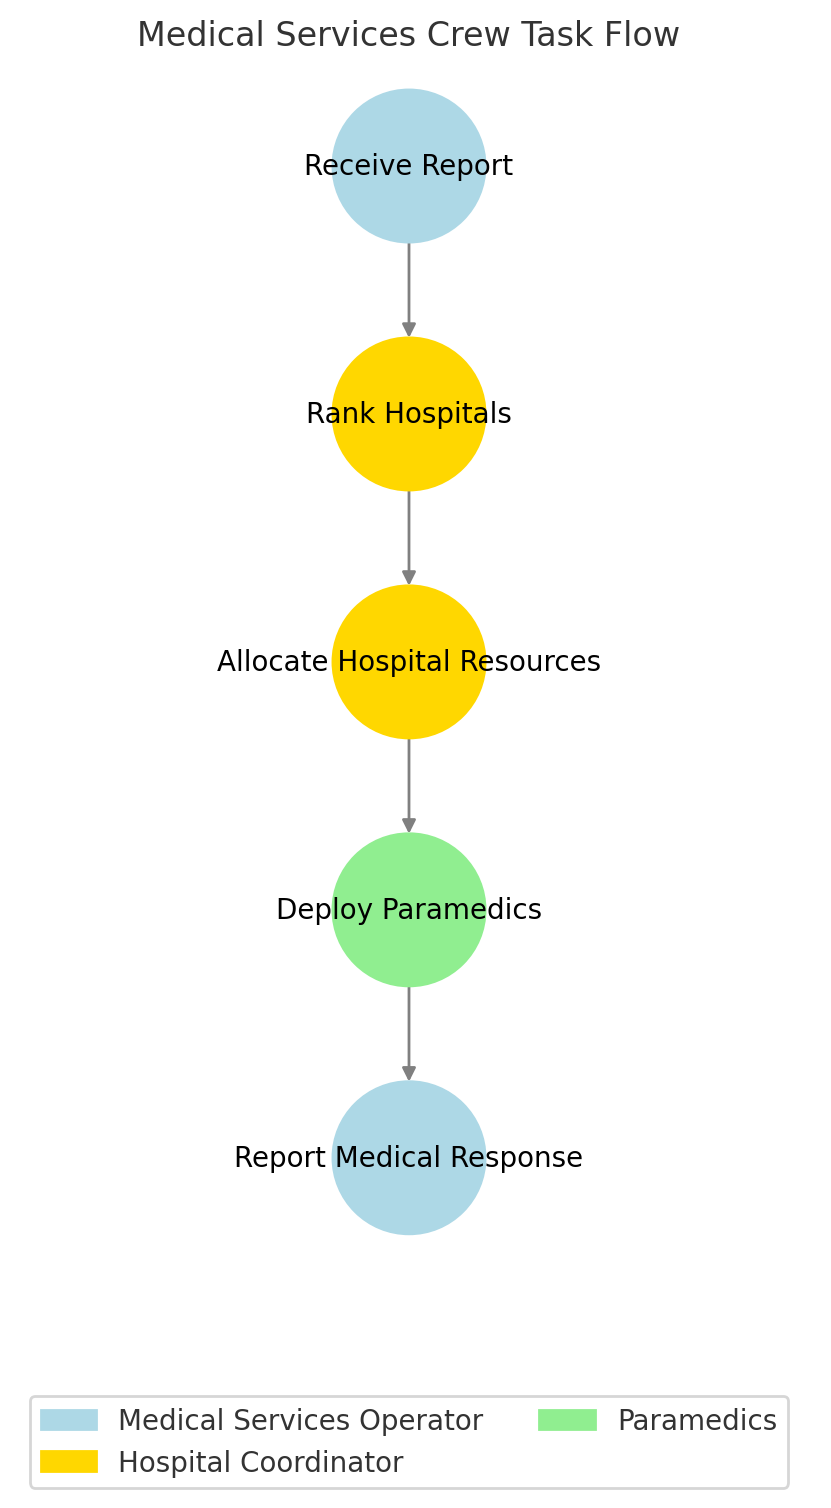
\includegraphics[height=\textheight]{figures/Medical_Services_Crew_Flow.png} 
\end{frame}

% Medical Services - Figure 2
\begin{frame}{Medical Services Outputs}
    \centering
    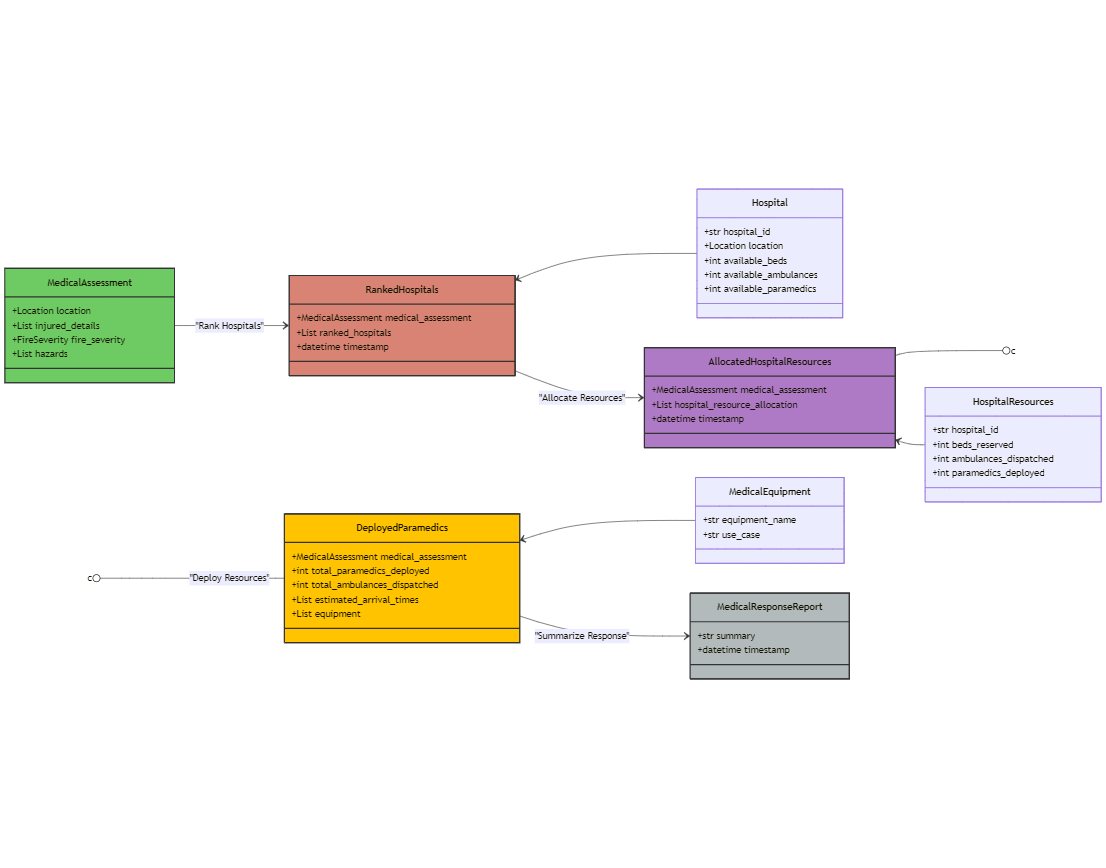
\includegraphics[width=\textwidth]{figures/MedicalServices_ClassDiagram.png}
\end{frame}
% Public Communications - Figure 1
\begin{frame}{Public Communications Process}
    \centering
    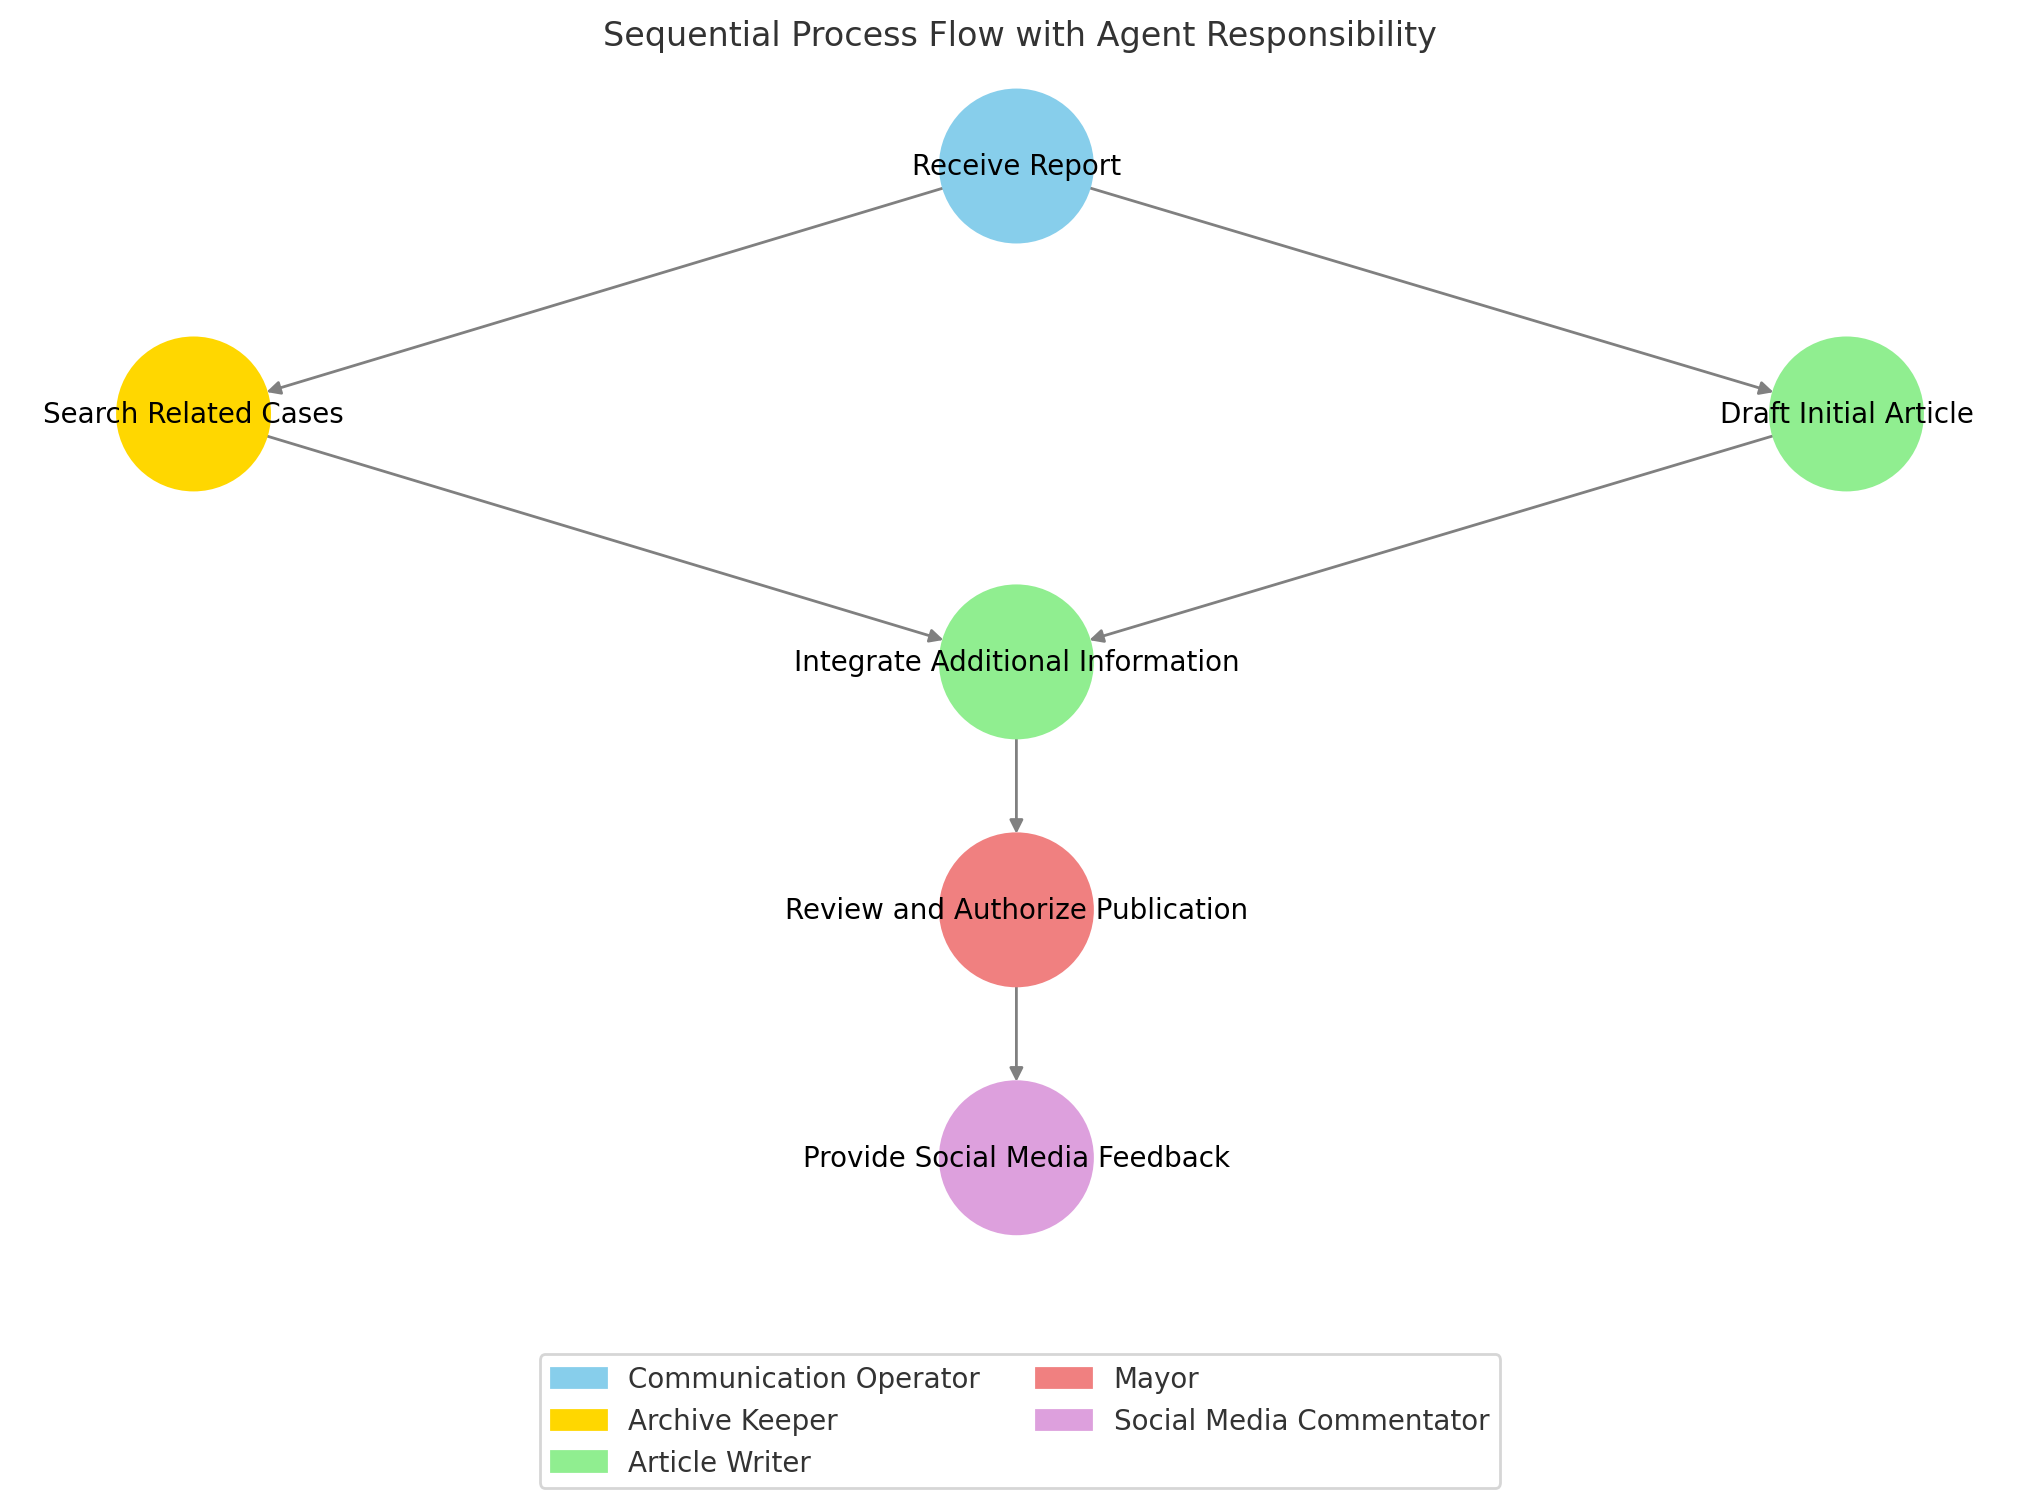
\includegraphics[width=\textwidth]{figures/PC-process.png} 
\end{frame}

% Public Communications - Figure 2
\begin{frame}{Public Communications Outputs}
    \centering
    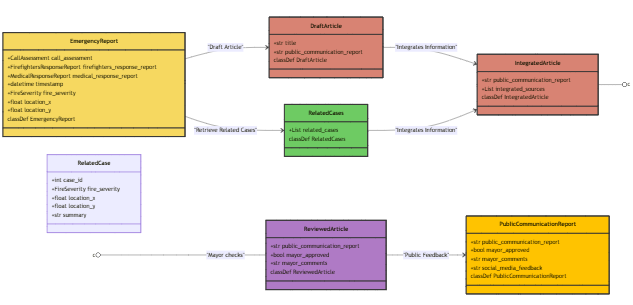
\includegraphics[width=\textwidth]{figures/PC-classDiagram.png}
\end{frame}
\section{Crew Interaction}
% Crew Interaction
\subsection{Emergency Planner Flow}
\begin{frame}{Emergency Planner Flow}
    \begin{columns}
        \begin{column}{0.45\textwidth}
            \begin{itemize}
                \item Crews coordinate through \textbf{centralized state}
                \item Flow manages \textbf{state} and \textbf{crew kickoffs}
                \item Use of \texttt{\_and}, \texttt{\_or} and \texttt{router} allow \textbf{complex ordering} and \textbf{parallelization}
                \item \textbf{Retry system} facilitates public communications
            \end{itemize}
        \end{column}
        \begin{column}{0.55\textwidth}
            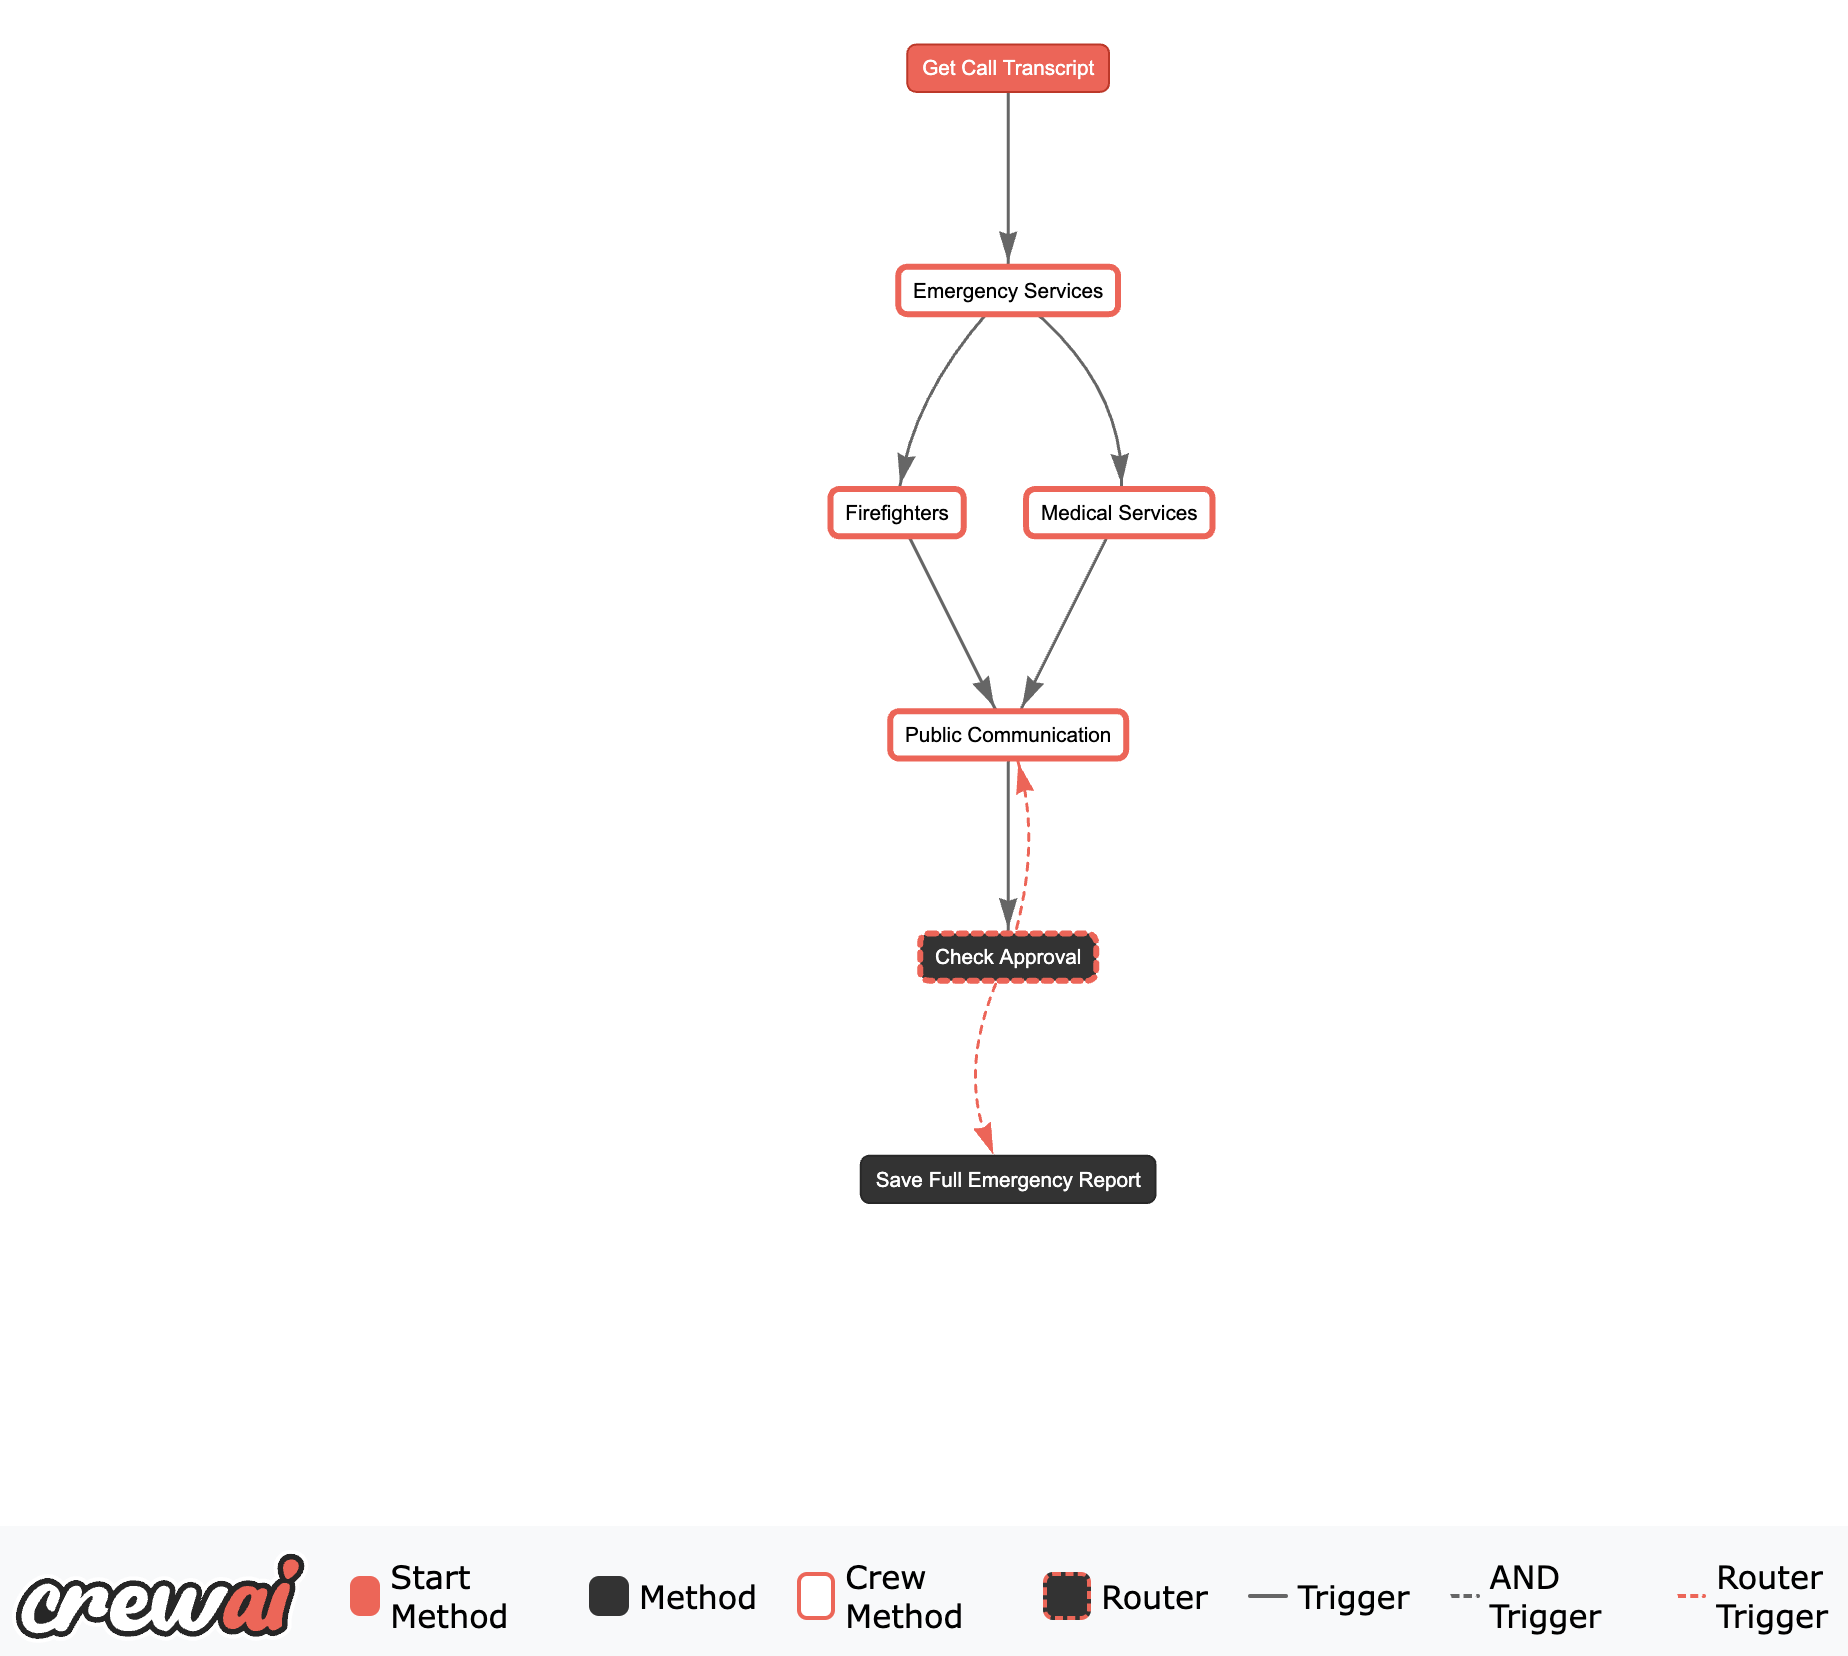
\includegraphics[width=\textwidth]{../figures/coordination_flow.png}
        \end{column}
    \end{columns}
\end{frame}

\subsection{Emergency Planner State}
\begin{frame}[fragile]{Emergency Planner State}
    \begin{lstlisting}[language=Python]
class EmergencyPlannerState:
    call_transcript: str | None
    call_assessment: CallAssessment | None
    firefighters_report: FirefightersReport | None
    medical_report: MedicalReport | None
    public_report: PublicReport | None
    retry_count: int = 0
    \end{lstlisting}
\begin{itemize}
    \item \texttt{call\_transcript}: The transcript of the emergency call
    \item \texttt{call\_assessment}: From \texttt{EmergencyServices} crew
    \item \texttt{firefighters\_response\_report}: From \texttt{Firefighters} crew
    \item \texttt{medical\_response\_report}: From \texttt{MedicalServices} crew
    \item \texttt{public\_communication\_report}: From \texttt{PublicCommunication} crew
    \item \texttt{mayor\_approval\_retry\_count}: Number of mayor approval attempts
\end{itemize}
\end{frame}


\section{Conclusion}
\begin{frame}{Conclusion}
    \begin{itemize}
        \item The \textbf{Emergency Services} crew establishes robust initial assessment and crew dispatching
        \item The \textbf{Firefighters and Medical Services} crews demonstrate effective parallel operation and complex processes
        \item The \textbf{Public Communications} crew generates useful summaries with mayor approval system and retry mechanisms
        \item A \textbf{centralized state management} with the CrewAI flow framework enables coordination between crews
        \item A \textbf{standardized reporting system} with structured outputs from each specialized crew is compiled into a single report
    \end{itemize}
\end{frame}

\begin{frame}
    \centering
    \vspace{2cm}
    {\Large Thank You!}
    \vspace{1cm}
    
    {\large Questions?}
\end{frame}

% References
\bibliographystyle{plain}
\section{References}
\begin{frame}{References}
    \nocite{*}
    \bibliography{references}
\end{frame}

\end{document}
